% vim:ft=tex nospell
\begin{block}{\large %
  CCSD(T):RPA for %
  H\textsubscript{2}O@[C\textsubscript{3}N\textsubscript{4}]%
  }
  138 atoms with $N_{\rm o}=292$. Embedded CCSD(T) calculations with
  up to $N_{\rm o}=40$ and $N_{\rm v}=800$\cite{schafer2021}.\\
  \begin{columns}
    \begin{column}{.49\linewidth}
      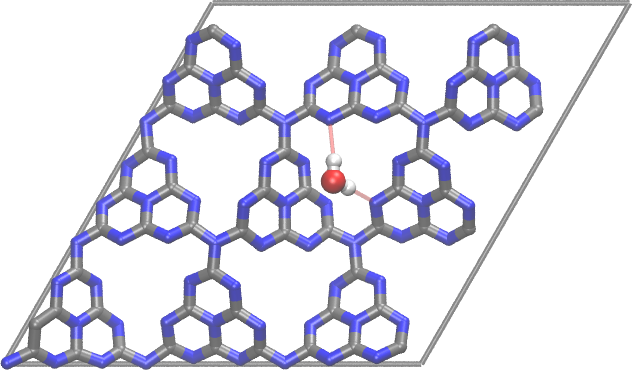
\includegraphics[width=\textwidth]{./figures/h2o_gc3n4_topview.png}\\
      \bigskip
      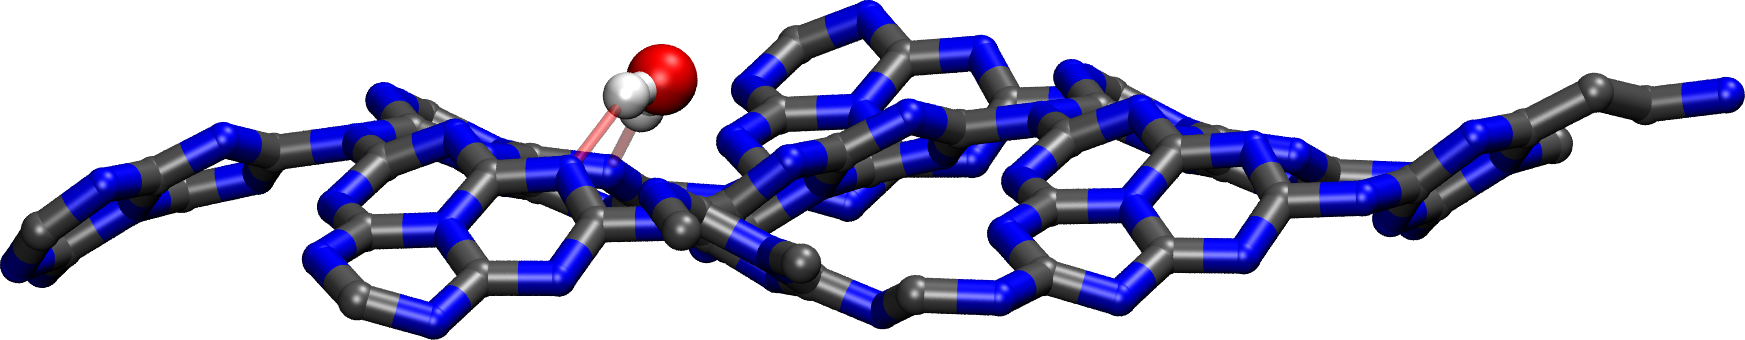
\includegraphics[width=\textwidth]{./figures/h2o_gc3n4_sideview.png}
    \end{column}
    %
    \begin{column}{.49\linewidth}
      \begin{tabular}{ c|c } 
        {\small Method } & {\small  E\textsubscript{ad} (kcal/mol) }\\
        \hline
        PBE & -8.1  \\ 
        PBE-D3 & -12.2 \\ 
        PBE-TS & -12.7 \\ 
        PBE0-MBD & -12.4 \\ 
        HF & -4.8 \\
        {\small  MP2:dMP2 } & -12.4 \\
        {\small  CCSD:RPA } & -10.7 \\
        {\small  CCSD(T):RPA } & -11.9
      \end{tabular}
    \end{column}
  \end{columns}
\end{block}
